\documentclass[12pt]{exam}         %% What type of document you're writing.

%%%%% Preamble

%% Packages to use

\usepackage{amsmath,amsfonts,amssymb}   %% AMS mathematics macros
\usepackage{lettrine}
\usepackage{graphicx}
\usepackage{tikz}

%% Title Information.

\title{Problems for Fun}
\author{Kedar Mhaswade}
\date{16 November 2020}


\begin{document}

\maketitle

\lettrine[lines=3]{T}{his} text consists of problems that should be attempted for fun. It is based on what we have learned
so far, however, that is just to be used as a guidance. Have fun. Find out what \emph{kind} of problems
are challenging and then perhaps work on the fundamentals.

Some points to keep in mind:
\begin{enumerate}
\item It may be a good idea to print this out on both sides of a paper and attempt the answers with a pen or pencil on a separate paper.
\item There are no points. A quiz may contain errors. If a question is unclear, be sure to get it clarified.
\item It is a quiz of sorts. The time is not really limited, but you should plan on focusing for about an hour each time you take the quiz.
\item Give each problem enough thought and time and then present your solutions.
\item Have fun. Hopefully, you will struggle to get through the problems. Perhaps you will make silly mistakes. Don't worry, it is all part of the game. You will get better only if you have fun doing it. Note that some problems are quite difficult and you may be stuck. Being stuck is okay.
\end{enumerate}

\paragraph{Problems}
\begin{questions}

\question
Multiply (see \cite{martin}) your phone number (disregard its area code) by 8. Write down the following three numbers:
\begin{enumerate}
\item Your phone number,
\item 8, and
\item The product of your phone number and 8.
\end{enumerate}
Add \emph{all} the digits in those three numbers. If the sum is more than one digit, add again. Continue this way until a single digit is reached.

What's the digit? What digit do you get with your friend's phone number? Why?

\question
If you had ten bananas (see \cite{martin}) and a monkey stole all but six, how many bananas would you have left?

\question
\begin{parts}
\part
If $100^\frac{1}{2} = x$, what is the value of $x$?
\part
What power (exponent) of $8$ is $32$? 
\end{parts}

\question
In how many different ways (see \cite{eom}) can the missing digits in this short
multiplication be completed?
\begin{equation*}
\begin{tabular}{r@{\;}l@{}}
$\square$ 6  \\
$\times$ $\square$  \\
\hline
$\square$ $2$ $8$\\
\end{tabular}
\end{equation*}

\question
How might you use the Pascal's triangle to find out $(a-b)^4$? When both $a$ and $b$ are same, can you verify the answer you get?

\question
In the wonderful state of Sunbathia, license plates of cars are all five characters. The first two characters are the letters of the English alphabet and each of the last three letters is a hexadecimal digit. How many total license plates are possible?

\question
Fill the grid so every row, column, and outlined region contains all the numbers 1 through 5 (See \cite{mtc}).
Hint: never guess!
\begin{figure}[htbp]
    \centering
    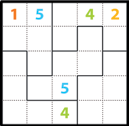
\includegraphics{sudoku.png}
    \caption{S for Sudoku}
\end{figure}

\question
A number of Puppies and another number of Kittens are in two pens. Two players take
turns making one of three possible moves: taking any number of puppies, or any number
of kittens, or the \emph{same number} of each. So, for example, if there are 8 puppies and 6 kittens,
a player could, in a move, take 4 puppies, or 2 kittens, or 3 puppies and 3 kittens.

One player decides the starting number of puppies and kittens and the other player decides who
goes first. The winner is the player who takes the last animal remaining.
\begin{center}
\tikz \draw (0,0) ellipse [x radius=30pt, y radius=20pt]; \hspace{0.5cm}
\tikz \draw (0,0) ellipse [x radius=30pt, y radius=20pt]; \\
Puppies \hspace{1cm} Kittens
\end{center}

For any starting number of puppies and kittens, is there an optimal strategy so one player is guaranteed to win? (See \cite{mtc})

\question
Are you convinced that the following statement is true?

``If the sum $s$ of the digits of a four-digit number $N$ is divisible by 3, then the number $N$ is divisible by 3''.

Make a sound argument using algebra.


\end{questions}

\begin{thebibliography}{00}
    \bibitem{martin} Gardner, Martin. MENTAL MAGiC Surefire Tricks to Amaze Your Friends. Dover Publications, 2009. 
    \bibitem{eom} Borovik Alexandre, Gardiner Tony. Essence of Mathematics. Open Book Publishers, 2019. 
    \bibitem{mtc} MT Circular. Fall 2019. Page 13.
\end{thebibliography}
\end{document}
